\subsection{Prinzip}
Die Haupt-Platine des Testroboters hat den Zweck den Großteil der benötigten Elektronik abzudecken. Das Erstellen von Schaltplan und Layout wurde mithilfe von KiCad realisiert. 
Da KiCad davor noch nie von uns verwendet wurde begann ein umfangreicher Lernprozess, mit vielen Stolpersteinen. 
\par\vspace{1em}
\noindent
Auf der Hauptplantine sollen der ESP32, das DFPlayer-Modul, Anschlüsse zur Servoansteuerung und Anschlüsse zur Wärmeansteuerung untergebracht werden. Zudem gibt es noch 
einen Spannungsregulator, der die 7,4V des Netzteils auf die für die Elektronik benötigten 5V hinunterregeln soll. Der gesamte Schaltplan ist in Abbildung \ref{fig:pcb:MP_all}
abgebildet. 

\subsection{Schaltplan}
\begin{figure}[H]
\centering
\includegraphics[angle = 90, width = 15cm]{images/PCBs/MP_all.pdf}
\caption{Schaltplan der Haupt-Platine des Testroboters}
\label{fig:pcb:MP_all}
\end{figure}
\newpage
\noindent

\subsubsection{Allgemeine Informationen zum Designprozess}
In KiCad ist es möglich eine Platine mit nahezujeden Bauteilen zu erstellen, da man Symbol- und Footprintdatein benutzerdefinert einfügen kann. 
Die Symboldatein sind für ein Erstellen des Schaltplans, die Footprints für das Layout. Auch beim Erstellen unserer Platinen mussten wir von dieser Anwendung 
Gebrauch machen. Die Symbole und Footprints von ESP und DFPlayer-Modul wurden von der Website SnapMagic \cite{snapeda_platform} heruntergeladen. SnapMagic bietet eine 
große Auswahl an Footprint- und Symboldatein zum freien Herunterladen an. 
\par\vspace{1em}
\noindent
Die Kreuze an den Pins von ESP und DFPlayer-Modul sind eine Kennzeichung in KiCad, dass diese Pins nicht benutzt werden. Diese zu setzten ist sehr wichitg, 
damit man von Schaltplan- ins Layoutdesign übergehen kann. 
\noindent
Das zweite Kriterium dafür sind die Powerflags, wie sie zum Beispiel bei Verbindungen wie V\_ESP, 3V3 und VCC zu sehen sind. Diese kennzeichenen in KiCad, 
dass diese Netze mit Spannung versorgt werden, obwohl keine für KiCad erkennbare Spannungsquelle angeschlossen ist. Sind diese nicht gegeben kann kein erfolgreicher 
ERC (Electrical Rule Checker) gemacht werden. 

\subsubsection{ESP32}
Der ESP32 wird mit einer Spannung von 5V am Pin für externe 5V versorgt. Das ist möglich, weil der ESP an disem GPIO-Pin einen internen Spannungsregler eingebaut hat welcher 
die 5V auf die 3V3 die der ESP braucht regelt \cite{esp32_devkitc_schematic}. Zusätzlich wurden noch 3 Stützkondensator zum Schutz des ESPs verbaut. 
Diese wurden mit den Werten 10nF, 1$\mu$F und 220$\mu$F dimensioniert, siehe Abbildung \ref{fig:pcb:MP_ESP}. Die ServoPWMx- Pins sind für die Servoansterung. Die SRXtoTX und STXtoRX für die
UART-Verbindung mit dem DFPlayer-Modul. HeatControl ist der Steuerungspin welcher die Wärmesimulation ein- und ausschaltet. Der PT100 Pin ist als Input-Pin für Daten des PT100 auf der Heat-Platine vorgesehen,
der 3.3V Ausgangspin versorgt diese Sicherungsschaltung auf der Heat-Platine. Mehr zur Wärmesimulation in Kapitel \ref{Warum?Heat}. 
\begin{figure}[H]
\centering
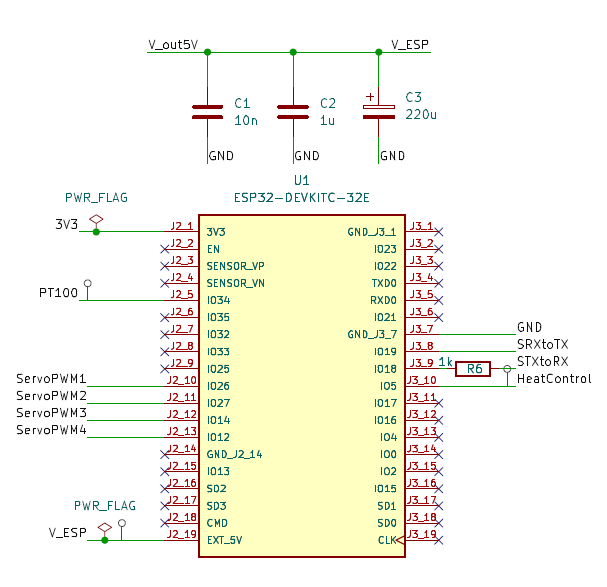
\includegraphics[width = 10cm]{images/PCBs/MP_ESP.png}
\caption{ESP auf der Hauptplantine}
\label{fig:pcb:MP_ESP}
\end{figure}
\noindent

\subsubsection{Spannungsregler}
Die Spannungsreglerschaltung wurde aus einer anderen Diplomarbeit unseres Betreuungslehrers übernommen. Das zentrale Element ist der Spannungsregler 
LM2596 \cite{lm2596_datasheet}. Das Textfeld neben der Schaltung ist eine Auflistung der zu verwendenden Vorwiderstände für die Diode, je nach gewünschter 
Ausgangsspannung. Der Messpunkt dient zur Überprüfung der Spannung nach dem Regeln. Die 5V am Ausgang der Spannungsreglerschaltung versorgen der ESP und das Player-Modul. Der Eingang sind die 7,4V 
des externen Netzteils diese werden mittels Schraubklemmen mit der Elektronik der Platine verbunden, siehe Abbildung \ref{fig:pcb:MP_vcc}.
Die Spannungsreglerschaltung ist in Abbildung \ref{fig:pcb:MP_voltage} veranschaulicht. 
\begin{figure}[H]
\centering
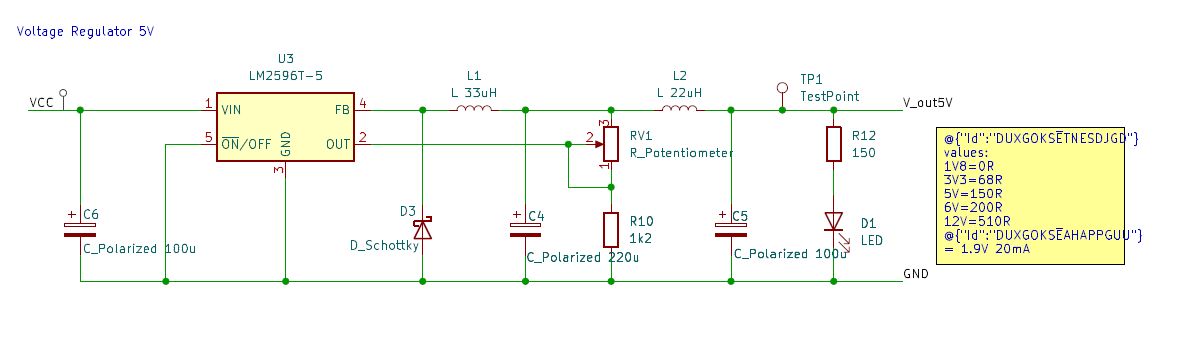
\includegraphics[width = 12cm]{images/PCBs/MP_voltage.png}
\caption{Spannungsreglerschaltung auf der Hauptplantine}
\label{fig:pcb:MP_voltage}
\end{figure}
\noindent

\begin{figure}[H]
\centering
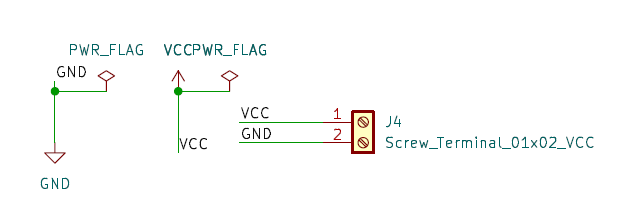
\includegraphics[width = 10cm]{images/PCBs/MP_vcc.png}
\caption{Spannungsversorgung auf der Hauptplantine über Netzteil}
\label{fig:pcb:MP_vcc}
\end{figure}
\noindent

\subsubsection{DFPlayer-Modul}
Der DFPlayer ist für die Audiosimulation von Wichtigkeit. Wie schon in Absatz \ref{Player} erklärt, kann man damit Audiodatein von der MicroSD-Karte 
decodieren und vom angeschlossenen Lautsprecher wiedergeben lassen. Die Verschaltung des Moduls auf der Platine ist sehr simpel. Die Versogung erfolgt über den 5V Output 
der Spannungsreglerschaltung, Ground (GND) ist mit dem allgemeinen GND verbunden. Für die Kommunikation mit dem ESP wird die UART-Schnittstelle genutzt. 
Dabei werden die TX (transmit) und RX (receive) immer mit dem jeweiligen Gegenstück verbunden:
\begin{itemize}
    \item RX (ESP) zu TX (Modul)
    \item TX (ESP) zu RX (Modul) 
\end{itemize}
Wichtig beim ESP ist es nicht die am ESP gekennzeichneten RX und TX zu benutzen. Diese sind für die USB-Seriall-Schnittstelle reserviert. Also zum Beispiel
für die Kommunikation während des Überspielen eines Programmcodes, oder zur Ausgabe von Debug-Meldungen über den Serialmonitor \cite{esp32_hardware_design_guidelines}.
Der Widerstand zwischen dem TX-Pin des Moduls und des RX-Pins des ESPs stellte sich später als unnötig heraus. Zuvor war er als Spannungsschutz gedacht, aber das DFPlayer-
Modul arbeitet intern mit einer Spannung von 3,3V und ist somit kein Problem für den ESP. Die Pins SPK1 und SPK2 sind die Anschlüsse für den Lautsprecher, sie
führen zu Schraubklemmen von denen aus die Kabel zum Lautsprecher geführt werden, siehe \ref{Ergebniss:Testroboter:verkabelung}. Zusehen ist die Verschaltung in Abbildung \ref{fig:pcb:MP_speaker}
\begin{figure}[H]
\centering
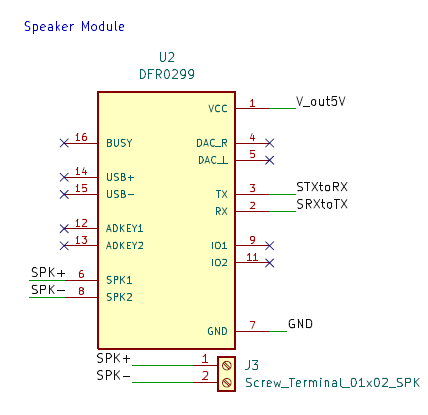
\includegraphics[width = 10cm]{images/PCBs/MP_speaker.png}
\caption{DFPlayer-Modul auf der Hauptplantine}
\label{fig:pcb:MP_speaker}
\end{figure}
\noindent

\subsubsection{Servoansteuerung}
Da die Servos mehr als 5V brauchen, werden sie über das Netzteil versorgt. Die Ansteuerung erfolgt jedoch über die PWM-Pins des ESP. Es wurde so vorgesehen dass die entsprechenden
Pins jeweils zu einer Schraubklemme führen, siehe \ref{fig:pcb:MP_servos}. Von dort werden sie dann mit Kabeln zu den Servos verbunden. 
\begin{figure}[H]
\centering
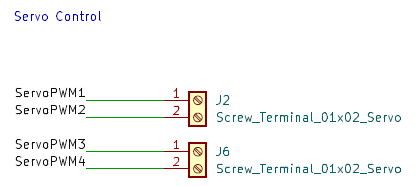
\includegraphics[width = 10cm]{images/PCBs/MP_Servo.png}
\caption{Servoansteuerung auf der Hauptplantine}
\label{fig:pcb:MP_servos}
\end{figure}
\noindent

\subsubsection{Wärmeansteuerung}
Auf der Haupt-Platine des Testroboters erfolgt nur die Ansteuerung der Wärmesimulation. Die eigentliche Eletrkonik der Wärmequelle ist auf eine zusätzliche 
Platine ausgelagert worden, siehe \ref{Heat Platinen}. Die Ansteuerung ist auf Abbildung \ref{fig:pcb:MP_heat} zu sehen. 
\begin{figure}[H]
\centering
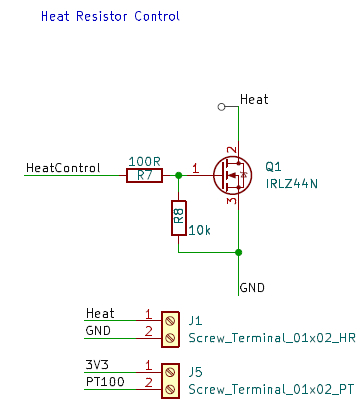
\includegraphics[width = 10cm]{images/PCBs/MP_heat.png}
\caption{Wärmeansterung auf der Hauptplantine}
\label{fig:pcb:MP_heat}
\end{figure}
\noindent
Die Ansteuerung erfogt mittels N-Kanal MOSFET, es wird der IRLZ44N \cite{irlz44n_datasheet} benutzt. Die Regulng erfolgt über einen GPIO Pin des ESPs. Ist dieser gesetzt wird der Stromkreis über GND geschlossen 
und es fließt Strom über die Heat Platin, dieser Aufbau ist in Abschnitt \ref{Warum?Heat} genauer beschreiben. Der 10k$\Omega$ Widerstand fungiert als Pull-Down 
Widerstand und der 100$\Omega$ Widerstand ist als Schutz den ESP vorgesehen. 
Zusätzlich sind in der Abbildung \ref{fig:pcb:MP_heat} auch noch die Schraubklemmen zur Verbindung der Heat-Platine mit der Haupt-Platine zu sehen. 

\subsection{Layout}

%\subsection{Versorgung der Platine} noch unsicher ob ich etwas dazu schreibe in dieser section

\section[Testroboter Heat-PCB]{Testroboter Heat-PCB \authorkatrin} \label{Heat Platinen}
\subsection{Prinzip} \label{Warum?Heat}
\subsection{Schaltplan}
\subsection{Layout}
%\subsection{Versorgung der Platine} noch unsicher ob ich etwas dazu schreibe in dieser section
\subsection{Platinenfertigung}